
\documentclass[12pt]{article}
\usepackage{amssymb}
\usepackage{graphicx}
\usepackage{placeins}

\title{Development of Real-Time Systems}

\begin{document}

\maketitle

\section*{Assignment 3}

In this assignment we will focus a bit more on the theoretical side. We will have a look at verifying real-time system by using the cyclic structured construct handled in the course and a simulation environment to automatically schedule a full timeline. The main purpose of the assignment is to expose the student to several ways of planning and verifying a real-time system in practice.

\section{Theory assignment}

The following part of assignment is a purely theoretical task that requires no additional tools. The task is to find the largest possible frame size for the cyclic structured scheduler by following requirements 1, 2 and 3 for finding the largest frame size. The following three task sets should be used:

\begin{enumerate}
\item $T_{1}(15,1,14)$ $T_{2}(20,2,26)$ $T_{3}(22,3)$
\item $T_{1}(4,1)$ $T_{2}(5,2,7)$ $T_{3}(20,5)$
\item $T_{1}(5,0.1)$ $T_{2}(7,1)$ $T_{3}(12,6)$ $T_{4}(45,9)$
\end{enumerate}

\subsection{Report 1}

This report shows the results with the first data: $T_{1}(15,1,14)$ $T_{2}(20,2,26)$ $T_{3}(22,3)$

\begin{itemize}

\item \textbf{Requirement 1}

$f\geq3$

\item \textbf{Requirement 2}

$f=\{22,20,15,11,10,5,4,3,2,1\}$

\item \textbf{Requirement 3}

\begin{tabular}{ l | l l l}
   & $T_{1}$ & $T_{2}$ & $T_{3}$ \\ \hline
  $22$ & $44 - 1 \nleq 14$ &    \\
  $20$ & $40 - 5 \nleq 14$ &  &  \\
  $15$ & $30 - 15 \nleq 14$ & & \\
  $10$ & $20 - 5 \nleq 14$ & & \\
  $5$ & $10 - 5 \leq 14$ & $10 - 5 \leq 26$  & $10 - 1 \leq 22$   \\
\end{tabular}

\item \textbf{Results}

The optimal frame size that fulfils the requirements is $f=5$.

\end{itemize}


\subsection{Report 2}

This report shows the results with the second data: $T_{1}(4,1)$ $T_{2}(5,2,7)$ $T_{3}(20,5)$

\begin{itemize}

\item \textbf{Requirement 1}

$f\geq5$

\item \textbf{Requirement 2}

$f=\{20,10,5,4,2,1\}$

\item \textbf{Requirement 3}

\begin{tabular}{ l | l l l  }
   & $T_{1}$ & $T_{2}$ & $T_{3}$ \\ \hline
  $20$ & $40 - 4 \nleq 4$ & &   \\
  $10$ & $20 - 2 \nleq 4$ & &   \\
  $5$ & $10 - 1 \nleq 4$ & &   \\
  $4$ & $8 - 4 \leq 4$ & $8 - 1 \leq 7$ & $8 - 4 \leq 20 $   \\

\end{tabular}

\item \textbf{Results}

In this case there is no frame size that fulfils the requirements since the candidate from the requirement 3 doesn't satisfies requirement 1. For making this system feasible, jobs from $T_{3}$, which have a execution time bigger than 4, should be split in smaller parts.

\end{itemize}


\subsection{Report 3}

This report shows the results with the third data: $T_{1}(5,0.1)$ $T_{2}(7,1)$ $T_{3}(12,6)$ $T_{4}(45,9)$

\begin{itemize}

\item \textbf{Requirement 1}

$f\geq9$

\item \textbf{Requirement 2}

$f=\{45,15,12,9,7,6,5,4,3,2,1\}$

\item \textbf{Requirement 3}

\begin{tabular}{ l | l l l l }
   & $T_{1}$ & $T_{2}$ & $T_{3}$ \\ \hline
  $45$ & $90 - 5 \nleq 5$ & & & \\
  $15$ & $30 - 5 \nleq 5$ & & & \\
  $12$ & $24 - 1 \nleq 5$ & & & \\
  $9$ & $18 - 1 \nleq 5$ & & & \\
  $7$ & $14 - 1 \nleq 5$ & & & \\
  $6$ & $12 - 1 \nleq 5$ & & & \\
  $5$ & $10 - 5 \leq 5$ & $10 - 1 \nleq 7$ & & \\
  $4$ & $8 - 1 \nleq 5$ & & \\
  $3$ & $6 - 1 \leq 5$ & $6 - 1 \leq 7$ & $6 - 3 \leq 12$ \\

\end{tabular}


\item \textbf{Results}


In this case there is no frame size that fulfils the requirements since the candidate from the requirement 3 doesn't satisfies requirement 1. For making this system feasible, jobs from $T_{3}$ and $T_{4}$, which have a execution time bigger than 3, should be split in smaller parts.

\end{itemize}

\section{Simulation assignment}

The assignment is to use a real-time simulator to verify feasibility of a set of tasks.

The following task sets and scheduler should be used:

\begin{enumerate}
\item $T_{1}(2, 0.5)$, $T_{2}(3, 1.2)$, $T_{3}(6, 0.5)$ and the RM scheduler 
\item $T_{1}(2, 0.5, 1.9)$, $T_{2}(5, 2)$, $T_{3}(1, 0.1, 0.5)$, $T_{4}(10, 5, 20)$ and the EDF scheduler
\end{enumerate}


\subsection{Report 1}

\begin{itemize}
\item \textbf{What is the utilization factor of the system and what is the value for Urm(3)}

Looking at the general tab, which is shown on figure \ref{ageneraltab}, the total utilization has a value of $0.7410$.

\begin{figure}[h]
\centering
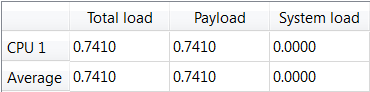
\includegraphics[scale=1]{figures/A_total_utilization}   
\caption{General tab of results window in the first simulation}
\label{ageneraltab}
\end{figure}
\FloatBarrier

This value is very similar with the theorical total utilization, which is calculated in the ecuation \ref{eqatotalutilization}

\begin{equation}\label{eqatotalutilization}
U= \frac{0.5}{2} + \frac{1.2}{3} + \frac{0.5}{6} = 0.7333 
\end{equation}

$U_{RM}(3)$ has been calculated using the ecuation \ref{equrm3}

\begin{equation}\label{equrm3}
U_{RM}(3)\ =\ 3·(2^{\frac{1}{3}}-1)=0.7798 
\end{equation}

\item \textbf{What is the minimum/maximum/average response time of all tasks?}

This data is shown on the task tab, which is presented on figure \ref{atasktab}.

\begin{figure}[h]
\centering
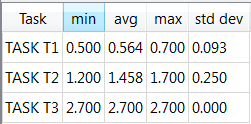
\includegraphics[scale=1]{figures/A_tasks}   
\caption{Task tab of results window in the first simulation}
\label{atasktab}
\end{figure}
\FloatBarrier

\item \textbf{Is any task missing the deadline? Which task? Where?}

There is no task missing its deadline. This can be seen in the log tab, which is presented on figure \ref{alogtab}.

\begin{figure}[h]
\centering
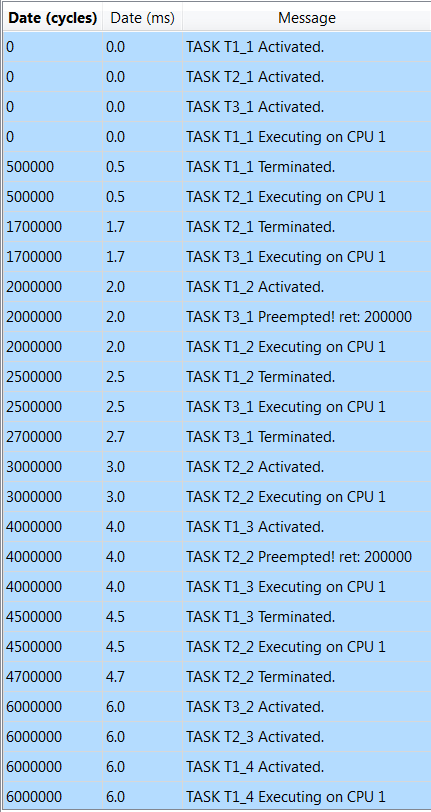
\includegraphics[width=0.7\textwidth]{figures/A_log}   
\caption{Log tab of results window in the first simulation}
\label{alogtab}
\end{figure}
\FloatBarrier

\item \textbf{If a deadline is missed, could it be avoided by changing the scheduler?}
\end{itemize}

There aren't missed deadlines in the simulation.   
   
\subsection{Report 2}

\begin{itemize}
\item \textbf{What is the utilization factor of the system and what is the value for Urm(4)}

Looking at the general tab, which is shown on figure \ref{bgeneraltab}, the total utilization has a value of $1.0000$.

\begin{figure}[h]
\centering
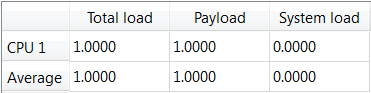
\includegraphics[scale=1]{figures/B_total_utilization}   
\caption{General tab of results window in the second simulation}
\label{bgeneraltab}
\end{figure}
\FloatBarrier

This value doesn't correspond with the theorical total utilization, which is calculated in the ecuation \ref{beqatotalutilization}

\begin{equation}\label{beqatotalutilization}
U= \frac{0.5}{2} + \frac{2}{5} + \frac{0.1}{1} + \frac{5}{10} = 1.25000 
\end{equation}

$U_{RM}(4)$ has been calculated using the ecuation \ref{equrm4}

\begin{equation}\label{equrm4}
U_{RM}(3)\ =\ 4·(2^{\frac{1}{4}}-1)=0.7568
\end{equation}

\item \textbf{What is the minimum/maximum/average response time of all tasks?}

This data is shown on the task tab, which is presented on figure \ref{btasktab}.

\begin{figure}[h]
\centering
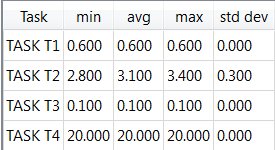
\includegraphics[scale=1]{figures/B_tasks}   
\caption{Task tab of results window in the second simulation}
\label{btasktab}
\end{figure}
\FloatBarrier

\item \textbf{Is any task missing the deadline? Which task? Where?}

Yes there is. Task 4 only satisfies its deadline on the first job and then always fails it and abort its execution. This is shown on the log of the simulation, which is presented on figure \ref{blogtab}. It can be seen that it execution exceeds the deadline at time 30.0 and successive.

\begin{figure}[h]
\centering
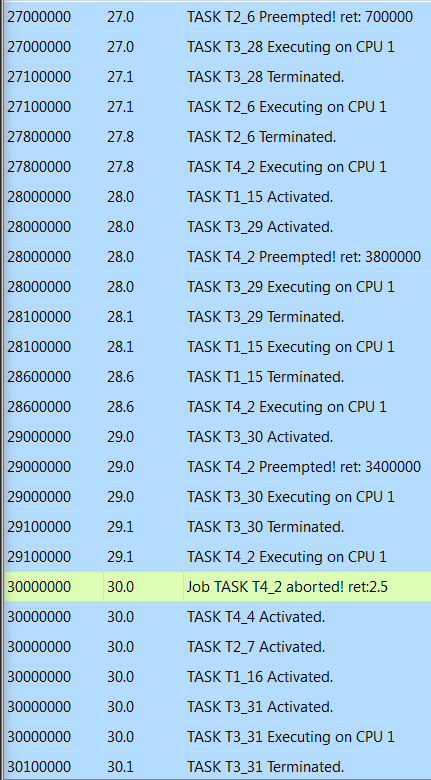
\includegraphics[width=0.7\textwidth]{figures/B_log}   
\caption{Log tab of results window in the second simulation}
\label{blogtab}
\end{figure}
\FloatBarrier

\item \textbf{If a deadline is missed, could it be avoided by changing the scheduler?}

In this case it can't, because as has been calculated in the first point, the theorical total utilization is $1.2500$, and this value is greater than $1.0000$

\end{itemize}
    
        
\end{document}